\documentclass{beamer}


% ==> mac template
%https://www.r-bloggers.com/2011/11/create-your-own-beamer-template/
%\usepackage{pgfcomp-version-0-65}
\usepackage{pgf}
\usepackage{tikz}
\usepackage{amsmath}
\linespread{1.25}
\usepackage{multicol}


% ==> math

\usepackage{mathtools}
\mathtoolsset{centercolon} % not work when using |mathpazo|
\DeclarePairedDelimiter\abs{\lvert}{\rvert}
\DeclarePairedDelimiterX\norm[1]\lVert\rVert{
	\ifblank{#1}{\:\cdot\:}{#1}
}
\def\set#1#2{\left\{#1 ~:~ #2\right\}}
\def\permil{\text{\hskip 0.3pt\englishfont\textperthousand}}


\DeclareMathOperator{\arccot}{cot}
\DeclareMathOperator{\arcsec}{arcsec}
\DeclareMathOperator{\arccsc}{arccsc}
\DeclareMathOperator{\lcm}{lcm}
\DeclareMathOperator{\ord}{ord}
\DeclareMathOperator{\sym}{sym}
\DeclareMathOperator{\tr}{trace}
\DeclareMathOperator{\spans}{span}
\DeclareMathOperator{\rank}{rank}
\DeclareMathOperator{\col}{col}
\DeclareMathOperator{\row}{row}
\DeclareMathOperator{\sign}{sign}
\DeclareMathOperator{\perm}{perm}
\DeclareMathOperator{\coef}{coef}
%\DeclareMathOperator{\proj}{proj}

\def\N{\mathbb N}
\def\Z{\mathbb Z}
\def\Q{\mathbb Q}
\def\R{\mathbb R}
\def\C{\mathbb C}
\def\F{\mathbb F}
\def\P{\mathbb P}

\def\L{\mathcal L}
\def\U{\mathcal U}

\def\labelitemi{$\circ$}
\def\inv{^{-1}}
\def\ang#1{\left\langle#1\right\rangle}
\def\tran{^\mathrm{T}}
\renewcommand{\vec}[1]{\mathbf{#1}}
\def\perc{^\perp}
\def\proj#1#2{\mathrm{proj}_{#2}{#1}}



\usepackage{bbold}
\let\altmathbb\mathbb
\AtBeginDocument{\let\mathbb\altmathbb}
% <==
% ==> color
\usepackage{color}

\definecolor{Ftitle}{RGB}{20, 0, 200}
\definecolor{Ftext}{RGB}{0,0,0}
\definecolor{Fenum}{RGB}{20, 70, 100}

\definecolor{StdTitle}{RGB}{26, 33, 141}
\definecolor{Descitem}{RGB}{20, 70, 100}
%\definecolor{StdTitle}{RGB}{20, 70, 100}
\definecolor{StdBody}{RGB}{213,24,0}

\definecolor{AlTitle}{RGB}{255, 190, 190}
\definecolor{AlBody}{RGB}{213,24,0}

\definecolor{ExTitle}{RGB}{201, 217, 217}
\definecolor{ExBody}{RGB}{213,24,0}


\setbeamercolor{normal text}{fg = Ftext}
\setbeamercolor{frametitle}{fg = Ftitle}
\setbeamercolor{title}{fg = Ftitle}
\setbeamercolor{section in toc}{fg = Ftitle}
\setbeamercolor{section in toc shaded}{fg = Ftitle}
\setbeamercolor{item}{fg = Fenum}
\setbeamercolor{subitem}{fg = Fenum}
\setbeamercolor{subsubitem}{fg = Ftitle}
\setbeamercolor{description item}{fg = Descitem}
\setbeamercolor{caption}{fg = Ftitle}
\setbeamercolor{caption name}{fg = Ftitle}

% Standard block
\setbeamercolor{block title}{fg = Descitem, bg = StdTitle!15!white}
\setbeamercolor{block body}{bg = StdBody!12!white}

% Alert block
\setbeamercolor{block title alerted}{bg = AlTitle}
\setbeamercolor{block body alerted}{bg = AlBody!5!white}

% Example block
\setbeamercolor{block title example}{bg = ExTitle}
\setbeamercolor{block body example}{bg = ExBody!5!white}

% <==
% ==> fonts
%\usefonttheme{professionalfonts}

% Font for the presentation title
\setbeamerfont{title}{size = \huge}

% Font of the frame titles
\setbeamerfont{frametitle}{size = \Large}
% <==
% ==> inner theme
\useinnertheme{circles}
\setbeamertemplate{itemize items}[circle]
\setbeamertemplate{enumerate items}[circle]
\setbeamertemplate{navigation symbols}{}

% ==> logo line
\newcommand{\LogoLine}{%
  \raisebox{-12mm}[0pt][0pt]{%
  \begin{pgfpicture}{0mm}{0mm}{0mm}{0mm}
    \pgfsetlinewidth{0.28mm}
    \color{gray!70!blue}
    \pgfline{\pgfpoint{-3 mm}{1mm}}{\pgfpoint{10.125 cm}{1mm}}
  \end{pgfpicture}}
}
\setbeamertemplate{headline}[text line]{\LogoLine}
% <==
% ==> logo
\setbeamertemplate{sidebar canvas right}{
  \vspace*{0 pt}\hspace*{-42 pt}%
  {
\includegraphics[height=40 pt]{../pic/mac.jpg}}
}
% <==
% ==> adjust title
\setbeamertemplate{frametitle}{
  \vspace*{3mm}\hspace*{-2mm}\insertframetitle
}
% <==
% ==> footline
\newcommand{\Ffootline}{%
  \insertsection % The left end of the footline
  \hfill
  \textit{MAC} % The center
  \hfill
  \insertframenumber/\inserttotalframenumber % And the right end
}

\setbeamertemplate{footline}{%
  \usebeamerfont{structure}
  \begin{beamercolorbox}[
    wd=\paperwidth,ht=2.25ex,dp=1ex
    ]{title in head/foot}%
    \tiny\hspace*{4mm} \Ffootline \hspace{4mm}
  \end{beamercolorbox}
}
% <==
% <==
% ==> title
% Title

\newcommand{\TitleLine}{%
\raisebox{-12mm}[0pt][0pt]{%
\begin{pgfpicture}{0mm}{0mm}{0mm}{0mm}
\pgfsetlinewidth{0.10mm}
\color{gray}
\pgfline{\pgfpoint{55mm}{0mm}}{\pgfpoint{55mm}{50mm}}
\end{pgfpicture}}}

\newcommand{\MyTitle}{%
\hspace*{60mm}\vspace{-25mm}
\centering \inserttitle}

% Subtitle
\newcommand{\MySubTitle}{%
\hspace*{60mm}\vspace{-25mm}
\centering \footnotesize \textit{\insertsubtitle}}

% Author
\newcommand{\MyAuthor}{
\hspace*{60mm}\vspace{-25mm}
\centering \insertauthor}

% Institute
\newcommand{\MyInstitute}{
\hspace*{60mm}\vspace{-25mm}
\centering \footnotesize \textit{\insertinstitute}}

% Date
\newcommand{\MyDate}{
\hspace*{60mm}\vspace{-25mm}
\centering \insertdate}



% We declare the image that will be used as the logo
\pgfdeclareimage[width = 0.20\paperwidth]{big}{../pic/mac.jpg}

\setbeamertemplate{title page}{\TitleLine
\hspace*{11mm}\vspace*{-60mm}
\begin{beamercolorbox}[wd=0.5\paperwidth,ht=0.13\paperwidth]{Title}
\pgfuseimage{big}
\end{beamercolorbox}
%
\begin{beamercolorbox}[wd=\paperwidth,ht=0.06\paperwidth]{Title}
\usebeamerfont{Title}%
\MyTitle
\end{beamercolorbox}
%
\begin{beamercolorbox}[wd=\paperwidth,ht=0.03\paperwidth]{Title}
\usebeamerfont{Title}%
\MySubTitle
\end{beamercolorbox}
%
\begin{beamercolorbox}[wd=\paperwidth,ht=0.06\paperwidth]{Title}
\usebeamerfont{Title}%
\MyAuthor
\end{beamercolorbox}
%
\begin{beamercolorbox}[wd=\paperwidth,ht=0.03\paperwidth]{Title}
\usebeamerfont{head/foot}%
\MyInstitute
\end{beamercolorbox}
%
\begin{beamercolorbox}[wd=\paperwidth,ht=0.07\paperwidth]{Title}
\usebeamerfont{Title}%
\MyDate
\end{beamercolorbox}}
% <==
% <==

%\usepackage{asymptote}
%\def\asydir{asydir}
% ==> preamble

%\usefonttheme[onlymath]{serif}
%\setbeamertemplate{navigation symbols}{}
%\usetheme{EastLansing}
%\usecolortheme{seagull}
%\setbeamertemplate{headline}{}
%\setbeamertemplate{footline}[frame number]{}



\usepackage{multicol}
\usepackage{tikz}
\title{\bfseries Properties of Real Numbers}
\author{Inger Jeng, Sivmeng HUN}
\institute{Student of MAC: Cohort II}
\date{08 August 2022}
% <==


\begin{document}


% ==> title
\begin{frame}[plain]
  \maketitle
\end{frame}
\begin{frame}[plain]{Content}
  \tableofcontents
\end{frame}
% <==
% ==> intro
\begin{frame}[plain]
  \begin{center}
    {\huge\color{blue} Introduction}
  \end{center}
\end{frame}
\section{Introduction}
\begin{frame}{Introduction}
  From previous group presentation we have constructed the
  set $\R$ from $\Q$. Now, we turn our attention to study and 
  explore some properties of $\R$.
\end{frame}
% <==
% ==> field
\section{$\R$ is an Ordered Field}
\begin{frame}[plain]
  \begin{center}
    {\huge\color{blue} $\R$ is an Ordered Field}
  \end{center}
\end{frame}
% ==> algebraic
\begin{frame}{Algebraic Properties}
  We won't talk much the detail here because it was already presented.
  Basically $\R$ has two operations, namely that of addition $(+)$ and
  multiplication $(\times)$. This makes $(\R, +,\times)$ a \emph{field.}
  In other words, $(\R,+)$ and $(\R^{\ast},\times)$ are Abelian groups.

\end{frame}
% <==
% ==> ordering
\begin{frame}{Ordering Properties}
  The ordering of $\R$ is the same as those in $\Q$.
  Moreover, $(\R, \leq)$ is an ordered field and also an extension
  from $(\Q, \leq)$.\\[0.3cm]
  %
  (working on it)
\end{frame}

% <==
% <==
% ==> uncount
\section{Uncountabiliy of $\R$}

\begin{frame}[plain]
  \begin{center}
    {\huge\color{blue} Uncountabiliy of $\R$}
  \end{center}
\end{frame}
% ==> definition
\begin{frame}{Countable and Uncountable}
  Let's recall the definition of countable sets.
  \pause
  \begin{definition}
    A set $S\subseteq\R$ is said to be countable if there
    exist a bijection $f$ from $\N$ to $S$.
    A set is called uncountable if it's not countable.
  \end{definition}
  \pause
  As shown in Group 3, the set $\Q$ is countable. 
  How about the set $\R$? 
\end{frame}
% <==
% ==> (0,1) uncount
\begin{frame}{$(0,1)$ is uncountable}
  \pause
  \begin{lemma}
    The interval $(0,1)$ is uncountable.
  \end{lemma}
  \pause
  \begin{block}{Proof.}
    We'll prove this by contradiction.
    \pause
    Assume on the contrary that $(0,1)$ is countable, hence
    there's a bijection map $f:\N\to (0,1)$. 
    \pause
    Thus every number in $(0,1)$ can be enumerated (listed) 
    in a table below. \\[0.3cm]
    \pause
    %
    The idea is to produce a number in $(0,1)$ that is not already
    placed on the table shown below.
  \end{block}
\end{frame}
\begin{frame}[plain]
  \begin{block}{(continued)}
    \begin{center}
      \begin{tabular}{l|l}
        $n$ & \multicolumn{1}{c}{$f(n)$}\\\hline
        1   & 0.\textcolor{blue}{1}12212411 $\dots$ \\
        2   & 0.0\textcolor{blue}{9}3240987 $\dots$ \\
        3   & 0.58\textcolor{blue}{7}103941 $\dots$ \\
        4   & 0.314\textcolor{blue}{4}14391 $\dots$ \\
        5   & 0.0981\textcolor{blue}{3}2081 $\dots$ 
        %6   & 0.69841\textcolor{blue}{0}012 $\dots$ 
      \end{tabular}
    \end{center}
    \pause
    Let $N=0.a_1a_2a_3a_4\dots$ where the $n$-th digit of $N$, namely $a_n$,
    is found by adding $1$ to the $n$-th digit of $f(n)$ in modulo $10$.
    \pause
    Thus, according to the table above we found
    \[ N=0.20854\dots \]
    \pause
    And from this construction, we see that $N\neq f(n)$ for all $n\in\N$.
  \end{block}
\end{frame}
\begin{frame}[plain]
  \begin{block}{(continued)}
    Thus this $N\in(0,1)$ is no where to be found in the table,
    a contradiction.\\[0.3cm]

    This shows that the interval $(0,1)$ is uncountable.
  \end{block}

  \pause
  Now because $(0,1)\subset\R$, we conclude that $\R$ is also uncountable.
  We have established the following theorem:
  \pause
  \begin{theorem}
    The set $\R$ is uncountable.
  \end{theorem}

\end{frame}
% <==
% <==
% ==> completeness
\section{Completeness of $\R$}
\begin{frame}[plain]
  \begin{center}
    {\huge\color{blue} Completeness of $\R$}
  \end{center}
\end{frame}
% ==> what is completeness
\begin{frame}
  What does \emph{completeness of $\R$} mean?
  \pause
  (Spoiler Alert ...) 
  \begin{theorem}[Completeness of $\R$]
    \pause Every Cauchy sequence converges.
  \end{theorem}
  \pause
  Let's first ask ourselves: \pause
  \begin{itemize}
    \item What is a \emph{sequence}?\pause
    \item What does it mean to \emph{converge}?\pause
    \item What is a \emph{Cauchy sequence}?\pause
  \end{itemize}

  So, first let's talk about sequence and convergence.

\end{frame}
% <==
% ==> def of convergence
\begin{frame}{Sequence}

  A sequence is a real valued-function whose domain is $\N$.
  The most crucial part of the study of sequence is that of 
  convergence.\\[0.3cm]
  \pause
  What should the definition of convergence be?\\[0.3cm]
  \pause
  Intuitively, convergence means $a_n$ gets 
  \emph{arbitrarily} close to a value $L$ for large enough $n$.
  \\[0.3cm]\pause

  \begin{center}
    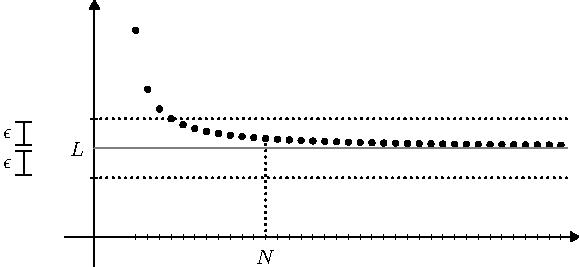
\includegraphics[scale=0.8]{converge.pdf}
  \end{center}

\end{frame}

\begin{frame}{Absolute Value}
  We define the absolute value by
  \[
    \abs{x}=
    \begin{cases}
      x &\text{if }x\geq 0;\\
      -x &\text{if }x<0
    \end{cases}
  \]
  The distance from $x$ to $y$ is given by $\abs{x-y}$.
  These are some properties of absolute value.
  \begin{block}{Properties}
    \begin{itemize}
      \item $\abs{x}\geq 0$
      \item $\abs{x+y}\leq \abs{x}+\abs{y}$
      \item $\abs{x-y}\geq \abs*{\abs{x}-\abs{y}}$
    \end{itemize}
  \end{block}
  %\begin{center}
  %\begin{tikzpicture}
  %\draw (-2,0)--(2,0);
  %\draw (-1,-0.1) node[below]{$x$}--(-1,0);
  %\draw (1.5,-0.1) node[below]{$y$}--(1.5,0);
  %\end{tikzpicture}
  %\end{center}
\end{frame}



\begin{frame}{Convergence}
  Okay, we have the language of distance. 
  The phrase ``$a_n$ is close to $L$'' can then be expressed by
  $\abs{a_n-L}<\epsilon$ for any small $\epsilon$.\\[0.3cm]

  Note that we only require it's true for larger and larger $n$.
  With all the ingredients at hand, we now present the

  \begin{definition}[Convergence]
    A sequence $(a_n)$ is said to converge to $L\in\R$ if 
    $\forall\epsilon>0,~ \exists N\in\N$ such that
    $\abs{a_n-L}<\epsilon$ for all $n\geq N$.
  \end{definition}

\end{frame}
% <==
% ==> monotone convergence
%\begin{frame}{Monotone Convergence}
  %%
  %Now how can we say for sure if a given sequence converge? The 
  %following theorem illustrates this.
  %\pause
  %%
  %\begin{theorem}
    %Let $(a_n)$ be a monotonic sequence. If $(a_n)$ is bounded,
    %then $(a_n)$ converges.
  %\end{theorem}
%\end{frame}
%\begin{frame}[plain]
  %\begin{proof}
    %We prove for the case when $(a_n)$ is an decreasing one, 
    %whereas the other case is proved similarly.  \\[0.3cm]
    %\pause

    %Now because $(a_n)$ is decreasing, the set $\{a_n~:~n\in\N\}$
    %has its infimum. Denote $a:=\inf a_n$. Let $\epsilon>0$, then
    %$a-\epsilon<a_n$ for all $n\in\N$, or 
    %\[-\epsilon<a_n-a\quad (\forall n\in\N).\]
    %%
    %\pause
    %Moreover, there is an $N\in\N$ such that $a+\epsilon>a_N$.
    %Since $(a_n)$ is decreasing, $a_n\leq a_N$ for all $n\geq N$. Thus
    %\[a_n-a\leq a_N-a<\epsilon, \quad (\forall n\geq N)\]
    %%
    %\pause
    %This means that $\abs{a_n-a}<\epsilon$ for all $n\geq N$.
    %\pause
    %Thus $\boxed{\lim a_n=a}$.
  %\end{proof}
%\end{frame}


% <==
% ==> Bolzano-Weierstrass
%\begin{frame}{Bolzano--Weierstrass theorem}
  %\begin{definition}
    %Let $(a_n)$ be sequence, and let $n_1<n_2<n_3<\cdots$
    %be an increasing sequence of positive integers. Then the sequence
    %\[
      %(a_{n_k}):~ a_{n_1},a_{n_2},a_{n_3},\dots
    %\]
    %is called a \emph{subsequence} of $(a_n)$.
  %\end{definition}
  %\pause
  %We present the amazing theorem
  %\pause
  %\begin{theorem}[Bolzano--Weierstrass]
    %Any bounded sequence has a convergent subsequence.
  %\end{theorem}
%\end{frame}
%\begin{frame}{Bolzano--Weierstrass theorem}
  %\begin{block}{Proof.}
    %We say that $a_m$ is a \emph{peek} term of $(a_n)$
    %if $a_m\geq a_n$ for all $n\geq m$.
    %\pause
    %Now, we have two cases to consider:\\[0.3cm]
    %\pause
    %%
    %\textbf{Case 1: } If there are infinitely many peek terms; \pause
    %then we let $a_{n_1}, a_{n_2}, a_{n_3},\dots$ be those peek terms. 
    %We obtain that $(a_{n_k})$ be an decreasing sequence, and it's bounded.
    %Thus by monotone convergence theorem, $(a_{n_k})$ converges.
    %%
  %\end{block}
%\end{frame}
%\begin{frame}[plain]{}
  %\begin{proof}[(continued)]
    %\textbf{Case 2: } If there are only finitely many peek terms; \pause
    %then we can let $a_m$ be the last peek term, and let $n_1=m+1$. \pause
    %Then there must exist an $n_2>n_1$ such that $a_{n_1}<a_{n_2}$, \pause
    %if otherwise we would obtain that $a_{n_1}$ be another peek term,
    %which is a contradiction because we are assuming that $a_m$ be 
    %the last peek term.\\[0.2cm]
    %%
    %\pause
    %Preceeding this procedure, we found $n_1<n_2<n_3<\cdots$ such that
    %\[a_{n_1}<a_{n_2}<a_{n_3}<\cdots\]
    %\pause
    %Thus, $(a_{n_k})$ is an increasing sequence and it's bounded.
    %Hence by monotone convergence theorem, we conclude that the subsequence
    %$a_{n_k}$ converges.
  %\end{proof}
%\end{frame}
% <==
% ==> cauchy
\begin{frame}{Cauchy Sequence}
  Now for the part we've been waiting for.
  We introduce
  \pause
  \begin{definition}[Cauchy Sequence]
    The sequence $(a_n)$ is called a \emph{Cauchy sequence} if 
    $\forall \epsilon>0,~ \exists N\in\N$ such that
    if $n,m\geq N$, then $\abs{a_n-a_m}<\epsilon$.
  \end{definition}
  \pause
  Our goal is to show that any Cauchy sequence converges. We'll break it
  into two little chunks.
  \pause
  For the remaining of this section, we denote $(a_n)$ be a Cauchy sequence.
\end{frame}
\begin{frame}{Cauchy sequence is bounded}
  \begin{lemma}
    Cauchy sequence is bounded.
  \end{lemma}
  \pause
  \begin{proof}
    We choose $\epsilon=1$ in the definition of Cauchy sequence to obtain
    that there's an $N\in\N$ such that (choose $m=N$)
    \begin{align*}
      &\abs{a_n-a_N}<1, \quad (\forall n\geq N)\\\implies
      &\abs{a_n}<1+\abs{a_N}
    \end{align*}
    \pause
    Then we denote 
    $M=\max\left\{\abs{a_1},\abs{a_2},\dots,\abs{a_{N-1}}, 1+\abs{a_N}\right\}$,
    \pause
    therefore, $\abs{a_n}\leq M$ for all $n\in\N$.
  \end{proof}
\end{frame}

\begin{frame}
  Now we know that $(a_n)$ is bounded. What can we say about bounded sequence?
  We borrow a theorem called \emph{Bolzano Weierstrass} theorem.
  \begin{definition}[Subsequence]
    Let $n_1<n_2<n_3<\cdots$ be increasing sequence of integers.
    We call $(a_{n_k})$ a subsequence of $(a_n)$.
  \end{definition}
  \begin{theorem}[Bolzano-Weierstrass]
    Any bounded sequence has a convergent subsequence.
  \end{theorem}
\end{frame}

\begin{frame}{Completeness of $\R$}
  \begin{theorem}[Completeness of $\R$]
    Any Cauchy sequence converges.
  \end{theorem}
  \pause
  \begin{block}{Proof.}
    From the above lemma $(a_n)$ is bounded, then it has a convergent
    subsequence (from Bolzano-Weierstrass). Suppose that 
    $(a_{n_k})$ be that convergent subsequence
    whose limit is $\lim a_{n_k}=a$. \\[0.3cm]
    \pause
    %
    Let an $\epsilon>0$, then there is $N\in\N$ such that
    $\abs{a_n-a_m}<\frac{\epsilon}{2}$ whenever $n,m\geq N$.
    \pause
    Because $(a_{n_k})\to a$ and $(n_k)$ is increasing, then
    there's $n_{k_0}>N$ such that 
    $\abs{a_{n_k}-a}<\frac{\epsilon}{2}$ whenever $k>k_0$.
  \end{block}
\end{frame}
\begin{frame}
  \begin{proof}[(continued.)]
    We obtain that for any $n\geq N$,
    \begin{align*}
      \abs{a_n-a}
      &\leq \abs{a_n-a_{n_k}}+\abs{a_{n_k}-a}\\
      &<\frac{\epsilon}{2}+\frac{\epsilon}{2}=\epsilon.
    \end{align*}
    \pause
    Thus $\lim a_n=a$. This completes the proof.
  \end{proof}
\end{frame}
% <==
% ==> advantage of completeness
\begin{frame}{What Does Completeness Mean?}
  Completeness of $\R$ is quite nice for it tells us that
  any Cauchy sequence has to have a limit in  $\R$.
  For instance, take the sequence
  \[a_n=1+\frac{1}{2^2}+\frac{1}{3^2}+\frac{1}{4^2}+\cdots+\frac{1}{n^2}.\]
  It's hard to prove that this sequence converges by guessing its limit.
  On the other hand, it's rather quite easy to prove it's a Cauchy sequence
\end{frame}
% <==

% <==
% ==> density
\section{Density of $\Q$ in $\R$}
\begin{frame}[plain]
  \begin{center}
    {\huge\color{blue} Density of $\Q$ in $\R$}
  \end{center}
\end{frame}
% ==> lim q_n=x
\begin{frame}{Density in language of sequence}
  Recall the Archimedean property that for any given $x\in\R$, 
  then there's an integer $n$ such that $n\geq x$.
  \pause
  In class, we've already exposed to the idea that $\Q$ is dense
  in $\R$. Today we're going to present the same thing but with
  different language.
  \pause
  \begin{theorem}
    Given any $x\in\R$, then there's a sequence $(q_n)\subset\Q$
    of rationals such that $\lim q_n=x$.
  \end{theorem}
\end{frame}
\begin{frame}
  \begin{block}{Proof.}
    The idea is to construct $(q_n)$. \pause
    Now for each $n\in\N$, notice the number $(xn-1)$ and $(xn+1)$ are 2 units apart,
    \pause
    thus there must be an integer $k\in\Z$ satisfying
    $xn-1<k<xn+1$, or equivalently
    \[x-\frac{1}{n}<\frac{k}{n}<x+\frac{1}{n}.\]
    \pause
    Without any doubt, we immediately denote $q_n:=\frac{k}{n}$, 
    thus we have constructed $(q_n)$ such that $\abs{q_n-x}<\frac{1}{n}$. 
    \pause
    With this sequence $(q_n)$ so constructed, we claim that its limit
    is exactly $x$.
  \end{block}
\end{frame}
\begin{frame}
  \begin{proof}[(continued.)]
    Let an $\epsilon>0$.\pause 
    From Archimedean property, we're pretty sure
    that there's an $N\in\N$ satisfying $N\geq\frac{1}{\epsilon}$.
    \pause
    Thus for any $n\geq N$, we obtain that
    \[ \abs{q_n-x}<\frac{1}{n}\leq\frac{1}{N}\leq\epsilon. \]
    This shows that $\lim q_n=x$ as advertised.
  \end{proof}
\end{frame}
% <==
% ==> density1 <=> density2
\begin{frame}{Density 1 $\iff$ Density 2}
  Right now, we have ways to state the density of $\Q$
  in $\R$. They are
  \pause
  \begin{theorem}[Density 1]
    Given any $x,y\in\R$ with $x<y$, then there exists a
    $q\in\Q$ such that $x<q<y$.
  \end{theorem}
  \pause
  \begin{theorem}[Density 2]
    Given any $x\in\R$, then there is a $(q_n)\subset\Q$
    such that $\lim q_n=x$.
  \end{theorem}
  \pause
  We have proved these two theorems independently by invoking
  the Archimedean property. 
  \pause
  We now will prove that these two
  are in fact equivalent. Namely, 
  \begin{center}
    Density 1 $\iff$ Density 2
  \end{center}
\end{frame}
\begin{frame}
  \begin{proof}[Proof. (Density 1 $\implies$ Density 2)]
    \pause
    The idea is the same, try to construct $(q_n)$. For each
    $n\in\N$, we could find $q_n\in\Q$ such that 
    $x<q_n<x+\frac{1}{n}$ (by Density 1).\\[0.3cm]
    \pause
    %
    Thus we have constructed $(q_n)$ such that 
    $\abs{q_n-x}<\frac{1}{n}$ for each $n\in\N$.
    \pause
    Using the same argument as the above proof, we could safely 
    conclude that $\lim q_n=x$ as expected.
  \end{proof}
\end{frame}
\begin{frame}[plain]
  \begin{proof}[Proof. (Density 2 $\implies$ Density 1)]
    \pause
    Let $x,y\in\R$ with $x<y$. Then by Density 2, we're sure that
    there's $(q_n)\subset\Q$ such that $\lim q_n=\frac{x+y}{2}$.
    \pause
    Let $r:=\frac{y-x}{2}>0$. 
    \pause
    \begin{center}
      \begin{tikzpicture}
        \def\tick{0.1}
        \draw (-2.2,0)--(2.2,0);
        \draw (0,-\tick)--(0,\tick) node[above]{$\frac{x+y}{2}$};
        \draw (-2,-\tick)--(-2,0) node[above]{$x$};
        \draw (2,-\tick)--(2,0) node[above]{$y$};
        \draw (-1.2,-\tick)--(-1.2,0)node[above]{$q_N$};

        \draw[|-|] (-2,-0.5)--(0,-0.5);
        \node[below] at (-1,-0.5) {$r$};
      \end{tikzpicture}
    \end{center}
    \pause
    Then there exists $N\in\N$ such that
    \begin{align*}
      \abs*{q_N-\frac{x+y}{2}}&<r\\
      \implies -r+\frac{x+y}{2}<q_N&<r+\frac{x+y}{2}\\
      \implies x<q_N&<y.
    \end{align*}
  \end{proof}
\end{frame}
% <==
% <==
% ==> why R
% ==> resource
% https://www.dpmms.cam.ac.uk/~wtg10/reals.html
% https://math.stackexchange.com/questions/1762147/why-do-we-study-real-numbers
% https://people.math.harvard.edu/~ctm/home/text/class/harvard/114/14/html/home/course/course.pdf
% <==
\section{Why Real Numbers?}
\begin{frame}[plain]
  \begin{center}
    {\huge\color{blue} Why Real Numbers?}
  \end{center}
\end{frame}
\begin{frame}{Why study on $\R$}
  Why do we bother to extend from $\Q$ to $\R$
  anyway? Well in real analysis, we would like to have 
  a rigorous way to the study of calculus. Namely, we
  need a \emph{good} definition of integral, differentiability,
  convergence, etc ... .
  \pause
  It turns out these objects were tied tightly to
  the concept of limit.\\[0.3cm]
\end{frame}
\begin{frame}{$\R$ is complete}
  How to study limit? The most convenient way is to study the limit
  of convergent sequences. \pause
  In $\R$, if a convergent sequence $(r_n)\subset\R$ then its 
  limit is closed, i.e. $\lim r_n\in\R$.
  \pause
  However, this is not always true in $\Q$. Take for instance
  a rational sequence
  \[1,  ~1.4, ~1.41, ~1.414, ~1.4142, ~1.41421, \dots \]
  yet their limit is $\sqrt 2\not\in\R$.\\[0.3cm]
  %
  \pause
  This is to say that $\R$ is complete, or to put it in another way,
  every \emph{Cauchy} sequence converges.
\end{frame}
% <==
% ==> ref
\section{Referrences}
\begin{frame}[plain]
  \begin{center}
    {\huge\color{blue} Referrences}
  \end{center}
\end{frame}
\begin{frame}{Referrences}
  (working on it).
\end{frame}
% <==


\end{document}
